\documentclass[11.5pt]{article}
\usepackage{stat110}

\title{Markov Chains}
\sectionnum{11}

\author{\justin}

% \SOLUTION

\begin{document}

\maketitle

\begin{notes}

\section*{Markov Chains}
A Markov Chain is a walk along a discrete \textbf{state space} \{$1, 2, \dots, M$\}. We let $X_t$ denote which element of the state space the walk is on at time $t$. The Markov Chain is the set of random variables denoting where the walk is at all points in time, $\{X_0, X_1, X_2, \dots \}$. Each $X_i$ takes on values that are in the state space, so if $X_1 = 3$, then at time 1, we are at state 3. 

What makes such a sequence of random variables a Markov Chain is the \textbf{Markov Property}, which says that if you want to predict where the chain is at at a future time, you only need to use the present state, and not any past information. In other words, the \emph{given the present, the future and past are conditionally independent}. 

Mathematically, this says: 
\[P(X_{n+1} = j | X_0 = i_0, X_1 = i_1, \dots, X_n = i_n) = P(X_{n+1} = j | X_n = i)\]
In words: Given that my history of states has been $i_0, i_2 \ldots i_n$, the distribution of where my next state will be doesn't depend on any of that history besides $i_n$, the most recent state. 
\section*{State Properties}
A state is either recurrent or transient.
\begin{itemize}
\item If you start at a \textbf{Recurrent State}, then you will always return back to that state at some point in the future.  \emph{You can leave, but you'll always return at some point.} 
\item Otherwise you are at a \textbf{Transient State}. There is some probability that once you leave you will never return. \emph{There's a chance that you'll leave and never come back}
\end{itemize}
A state is either periodic or aperiodic.
\begin{itemize}
\item If you start at a \textbf{Periodic State} of period $k$, then the GCD of all of the possible number steps it would take to return back is  $k$ (which should be $> 1)$.
\item Otherwise you are at an \textbf{Aperiodic State.} The GCD of all of the possible number of steps it would take to return back is 1.
\end{itemize}


\section*{Transition Matrix}
Element $q_{ij}$ in square transition matrix Q is the probability that the chain goes from state $i$ to state $j$, or more formally:
\[q_{ij} = P(X_{n+1} = j | X_n = i)\]

To find the probability that the chain goes from state $i$ to state $j$ in $m$ steps, take the $(i, j)^\textnormal{th}$ element of $Q^m$.
\[q^{(m)}_{ij} = P(X_{n+m} = j | X_n = i)\]
If $X_0$ is distributed according to row-vector PMF $\vec{p}$ (e.g. $p_j = P(X_0 = i_j)$), then the marginal PMF of $X_n$ is $\vec{p}Q^n$.



\section*{Chain Properties}
A chain is \textbf{irreducible} if you can get from anywhere to anywhere. An irreducible chain must have all of its states recurrent. A chain is \textbf{periodic} if any of its states are periodic, and is \textbf{aperiodic} if none of its states are periodic. In an irreducible chain, all states have the same period. \\

A chain is \textbf{reversible} with respect to $\vec{s}$ if $s_iq_{ij} = s_jq_{ji}$ for all $i, j$.  A reversible chain running on $\vec{s}$ is indistinguishable whether it is running forwards in time or backwards in time. Examples of reversible chains include random walks on undirected networks, or any chain with $q_{ij} = q_{ji}$, where the Markov chain would be stationary with respect to $\vec{s} = (\frac{1}{M}, \frac{1}{M}, \dots, \frac{1}{M})$. \\

\textbf{Reversibility Condition Implies Stationarity} - If you have a PMF $\vec{s}$ on a Markov chain with transition matrix $Q$, then $s_iq_{ij} = s_jq_{ji}$ for all $i, j$ implies that $s$ is stationary.


\section*{Stationary Distribution}

Let us say that the vector $\vec{p} = (p_1, p_2, \dots, p_M)$ is a possible and valid PMF of where the Markov Chain is at at a certain time. We will call this vector the stationary distribution, $\vec{s}$, if it satisfies $\vec{s}Q = \vec{s}$. As a consequence, if $X_t$ has the stationary distribution, then all future $X_{t+1}, X_{t + 2}, \dots$ also has the stationary distribution. 
\begin{itemize}
\item If a Markov Chain is irreducible, then it has a unique stationary distribution. In addition, all entries of this stationary distribution are non-zero (which could have been inferred from the fact that all states are recurrent).
\begin{itemize}
\item \textbf{Counterexample: } In the Gambler's Ruin problem, which is not irreducible, what ultimately happens to the chain can either be that one's money is always $0$ or always $N$. 
\end{itemize} 
\item If a Markov Chain is irreducible \textbf{and} aperiodic, then it has a unique stationary distribution $\vec{s}$ and $$ \lim_{n \to \infty} P(X_n = i) = \vec{s}_i$$
 meaning that the chain \textit{converges} to the stationary distribution. 
\begin{itemize}
\item \textbf{Counterexample: } Imagine a Markov chain which is just a cycle, and hence is periodic. Then, depending on where we start, $P(X_n = i)$ will be either 0 or 1 deterministically, and surely won't converge to the stationary distribution, which is uniform across all nodes in the cycle. 
\end{itemize}
\end{itemize}

For irreducible, aperiodic chains, the stationary distribution exists, is unique, and $s_i$ is the long-run probability of a chain being at state $i$. The expected number of steps to return back to $i$ starting from $i$ is $1/s_i$ To solve for the stationary distribution, you can solve for $(Q' - I)(\vec{s})' = 0$. The stationary distribution is uniform if the columns of $Q$ sum to 1.



\section*{Random Walk on Undirected Network}
If you have a certain number of nodes with undirected edges between them, and a chain can pick any edge uniformly at random and move to another node, then this is a random walk on an undirected network. The stationary distribution can be easily calculated. Let $d_i$ be the degree of the $i$th node, meaning the number of edges connected to this node. Then, we have: 
$$ \vec{s}_i = \frac{d_i}{\sum_i d_i}$$

For example, in the below graph:
\begin{center}
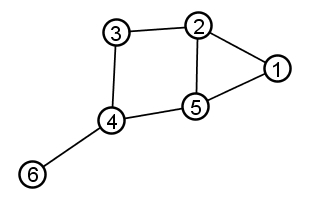
\includegraphics[scale=0.5]{nodes.jpg}
\end{center}

The stationary distribution would be proportional to: 
$(w_1, w_2, w_3, w_4, w_5, w_6) = (2, 3, 2, 3, 3, 1)$ and therefore, it would be $\left(\frac{2}{14},\frac{3}{14},\frac{2}{14},\frac{3}{14},\frac{3}{14},\frac{1}{14} \right)$

\end{notes}

\section*{Practice Problems} 

\begin{exercise}{Two-State Markov Chain}
Suppose $X_n$ is a two-state Markov chain with transition matrix

\[
Q = \bordermatrix{~ & 0 & 1 \cr
                  0 & 1-\alpha & \alpha \cr
                  1 & \beta & 1-\beta \cr}
\]
\begin{enumerate}
	\item Find the stationary distribution $\vec{s} = (s_0, s_1)$ of $X_n$ by solving $\vec{s} Q = \vec{s}$. 
	\item Show that this Markov Chain is reversible under the stationary distribution found in part (a)
	\item Let $Z_n = (X_{n-1}, X_n)$. Is $Z_n$ a Markov chain? If so, what are the states and transition matrix?
\end{enumerate}
\end{exercise}

\begin{solution}{5}
\begin{enumerate}
\item By solving $\vec{s} Q = \vec{s}$, we have that
$$s_0 = s_0 (1 - \alpha) + s_1 \beta \textrm{ and } s_1 = s_0 \alpha + s_1 (1 - \beta)$$
And by solving this system of linear equations, it follows that $\vec{s} = \paren{\frac{\beta}{\alpha + \beta}, \frac{\alpha}{\alpha + \beta}}$.

\item To verify the validity of a stationary distribution for a chain, we just need to show that $s_i q_{ij} = s_j q_{ji}$, which is done if we can show that $s_0 q_{01} = s_1 q_{10}$. We have that
$$s_0 q_{01} = \frac{\alpha\beta}{\alpha + \beta} = s_1 q_{10}$$
which satisfies our reversibility condition and verifies our stationary distribution from part (a).

\item Yes, $Z_n$ is a Markov Chain because conditional on $Z_n$, $Z_{n+1} \indep Z_{n-1}$. This is because the components of $Z_{n+1}$ and $Z{n-1}$ are either constants conditioned in $Z_n$ or independent of each other given that $X_n$ is a Markov Chain.

The states are given as $\{ (0, 0), (0, 1), (1, 0), (1, 1) \}$. The transition matrix is given as
\[
Q = \bordermatrix{   ~   & (0, 0) & (0, 1) & (1, 0) & (1, 1) \cr
                  (0, 0) & 1-\alpha & \alpha & 0 & 0 \cr
                  (0, 1) & 0 & 0 & \beta & 1-\beta \cr
                  (1, 0) & 1-\alpha & \alpha & 0 & 0 \cr
                  (1, 1) & 0 & 0 & \beta & 1-\beta \cr
                 }
\]
\end{enumerate}
\end{solution}

\begin{exercise}{Symmetrical Chain} 
A Markov chain $X_0,X_1, X_2\ldots$ with state space $\{3,2,1,0,1,2, 3\}$ proceeds as follows. The chain starts at $X_0 = 0$. If $X_n$ is not an endpoint ($-3$ or $3$), then $X_{n+1}$ is
$X_n +1$ or $X_n -1$, each with probability $1/2$. Otherwise, the chain gets reflected off the endpoint, i.e., from 3 it always goes to 2 and from $-3$ it always goes to $-2$. A diagram
of the chain is shown below.\begin{center}
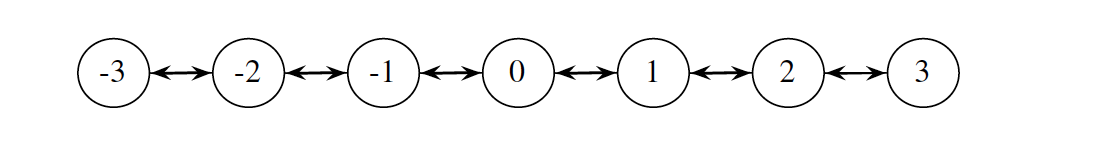
\includegraphics[scale=0.5]{markov1.png}
\end{center}
\begin{enumerate}
\item Is $|X_0|, |X_1|, |X_2|, \ldots$ a Markov Chain? 

\item Define the sign function $S(x)$ as follows: 
\[ S(x) = \begin{cases} 
      1 & x > 0 \\
      0 & x = 0 \\
      -1 & x < 0
   \end{cases}
\]

Is $S(X_0), S(X_1), S(X_2), \ldots$ a Markov Chain? 

\item Find the stationary distribution of the original chain: $X_1, X_2, X_3 \ldots$

\item Find a simple way to modify some of the transition probabilities $q_{ij}$ for $i,j \in \{-3, 3\}$ to make the stationary distribution of the modified chain uniform over the states.
\end{enumerate}

\end{exercise}


\begin{solution}{5.5} 
\vspace{-0.5em}
\begin{enumerate}
\item Yes it is a Markov chain with state space $\{0, 1, 2, 3\}$. We need to check that this new chain satisfies the Markov property. If we are given that $|X_n| = 1$, then regardless of what $|X_{n-1}|, |X_{n-2}|, \ldots$ are, we know that there is a $1/2$ chance $|X_{n+1}|$ will be 0 and a $1/2$ chance that it will be $2$. A similar argument can be made for all the states, and thus this chain satisfies the Markov property. 

\item We will show that this is not a Markov chain because it does not satisfy the Markov property. In general, when showing that something does or does not satisfy the Markov property, it is a good idea to ask yourself: "If I knew more than just the \textit{one} previous state, would that help me make a more informed decision about what the next state is?". 

In this case, if I told you that the last three states $S(X_{n-2}), S(X_{n-1}), S(X_n)$ were $0,1,1$, then we know that the chain is at $2$, i.e. $X_n = 2$. This means that $P(S(X_{n+1}) = 0) = 0$ because we can't jump from 2 to 0. However, if I told you that the last two states $S(X_{n-1}), S(X_n)$ were $0$ and $1$, then you would know that $X_n = 1$ and say that $P(S(X_{n+1}) = 0) = 1/2$. Thus, the Markov property is not satisfied because even though in both situations $S(X_n) = 1$, we had different probabilities for $P(S(X_{n+1}) = 1)$. 

\item We see that this is simply a random walk on an undirected graph, so the stationary distribution is proportional to the degrees of each of the states. The degrees are: $(1, 2, 2, 2, 2, 2, 1)$, and so the stationary distribution is: $\vec{s} = (1/12, 1/6, 1/6, 1/6, 1/6, 1/6, 1/12)$ 

\item If we could somehow get all the states to have the same degree, then the stationary distribution would be uniform across all states. Therefore, all we need to do is connect states 3 and -3 together, so that there is a $1/2$ chance at 3 to go to $2$ or $-3$, and equivalently for $-3$. 
\end{enumerate}
\end{solution} 

%%%%%%%%%%%%%%%%%%%%%%%%%%%%%%%%%%%%%%%%%%%%%%%%%%%%%%%%%%%

\begin{exercise} {Not a Markov Chain}
A Markov chain has two states, $A$ and $B$, with transitions as follows:
\begin{center}
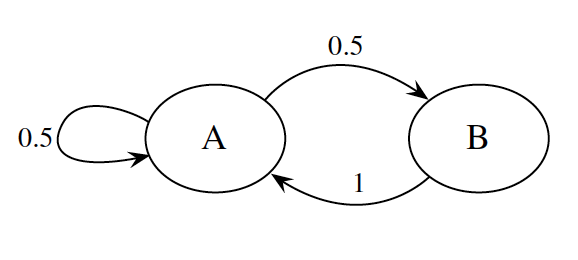
\includegraphics[scale=0.6]{markov2.png}
\end{center}

Suppose we do not get to observe this Markov chain, which we'll call $X_1, X_2, \ldots$.  Instead, whenever the chain transitions from $A$ back to $A$, we observe a 0, and whenever it changes states, we observe a 1. Let the sequence of 0's and 1's be called $Y_0, Y_1, Y_2, \ldots $
For example, if the X chain starts out as
$$A, A, B, A, B, A, A, \ldots$$
then the Y chain starts out as
$$0, 1, 1, 1, 1, 0, \ldots$$

\begin{enumerate}
\item Show that $Y_0, Y_1, Y_2, \ldots$ is not a Markov Chain. 

\item In the past, when we have encountered processes that are not directly Markov chains, our remedy was to create a new state $Z_n$ which would represent not only the current state $X_n$ that the chain is on, but also remember the past $m$ states. Thus, $Z_n$ is not just one state, but a tuple of states that represent the chain's history: 
$$ Z_n = \left(X_n, X_{n-1}, X_{n-2} \ldots X_{n - (m-1)} \right)$$
Show that such a trick will not work for $Y_0, Y_1, Y_2\ldots$. That is, no matter how large $m$ is, $\{Z_n\}$ will never be a Markov Chain. 
\end{enumerate}
\end{exercise}

\begin{solution} {5} 
\vspace{-0.5em}
\begin{enumerate}
\item We will show that knowing the chain outputted a 1 is not enough information to give the probability of the chain outputting 1 again on the next iteration. This is true because if the most recent sequence of outputs have been $0,1$, then the chain is clearly at $B$ in which case the probability of it outputting $1$ next is 1. However, if the chain's outputs had been $0,1,1$, then we know that the chain is at state $A$ in which case the probability of the next output being 1 (and hence the next state be B) is only $1/2$. 

\item The problem is saying that no finite amount of "memory" in this Markov chain is enough to be able to give a unique set of probabilities for the next output being $0$ or $1$, given a history of $m$ outputs. 

We notice that $1$'s in this Markov chain output always come in pairs. Assuming that you start at state A (which is valid because state A is recurrent), we see that outputting a $1$ means that another $1$ must follow. 

Suppose again that we're in the situation where out last output has been $1$. From the above fact that $1$'s always come in pairs, we can reason that it's not the number of $1$'s that have been outputted in the recent past that matters, but rather its parity (i.e even or odd). If a 0 is followed by an even number of $1$'s, then we know that the chain is at state $A$ so the probability of outputting either a $1$ or $0$ is $1/2$. If the number of $1$'s following that first $0$ is odd, then we know that the next output must be $1$ with probability 1.  

No amount of memory $m$ can completely capture the parity of the number or $1$'s that came before. This doesn't mean that there doesn't exist some clever way to create states such that this sequence of $0$'s and $1$'s becomes a Markov chain. Rather, this conclusions says that this one particular technique (remembering the past $m$ states) does not work in this case. 

\end{enumerate}
\end{solution}
%%%%%%%%%%%%%%%%%%%%%%%%%%%%%%%%%%%%%%%%%%%%%%%%%%%%%%%%%%%

\begin{exercise} {Balls and Urns} 
There are two urns with a total of $2N$ distinguishable balls. Initially, the first urn has $N$ white balls and the second urn has $N$ black balls. At each stage, we pick a ball at random from each urn and interchange them. Let $X_n$ be the number of black balls in
the first urn at time $n$. This is a Markov chain on the state space $\{0,1, 2, \ldots N\}$. 

\begin{enumerate}
\item 
Give the transition probabilities of the chain.

\item Set up, but do not evaluate, one or more equations that you would use to prove that $$\vec{s}_i = \frac{{N \choose i}{N \choose {N - i} }}{{2N \choose N}}$$ is the stationary distribution for the above Markov Chain. 

\textbf{Extension: } Show that the equation(s) you set up for part (b) are in fact true.
\end{enumerate}
\end{exercise} 

\begin{solution}{3} 
\vspace{-0.5em}
\begin{enumerate}
\item When asked to give transition probabilities, you must specify them for all pairs of $i,j$. Most of them, however, will be 0, but we need to specify those explicitly. 

For $|i - j| > 1$, we know that $p_{ij}$, the transition probability from state $i$ to state $j$ is 0. Thus, all we need to calculate is $p_{i,i}, p_{i,i+1}, p_{i, i-1}$. 

Here is a convenient table representing the number of balls of each color in each urn:  
\begin{center}
\begin{tabular}{ccc}
& First Urn & Second Urn \\ 
\hline
Black & $i$  & $N-i$ \\ 
White & $N-i$ & $i$ 
\end{tabular} 
\end{center}

The probability that the number of black balls in the first urn doesn't change is: 

$$ p_{i,i} = \pfrac{i}{N}\pfrac{N-i}{N} + \pfrac{N-i}{N} \pfrac{i}{N} = \frac{2i(N-i)}{N^2}$$

where the first term represents the probability of swapping two black balls, and the second term is the probability of swapping two white balls. 

$$ p_{i, i+1} = \pfrac{N-i}{N} \pfrac{N-i}{N} = \pfrac{N-i}{N}^2$$
because we need to swap a white ball from Urn 1 with a black ball from urn 2. 

Finally: 

$$ p_{i, i-1} = \pfrac{i}{N}^2$$ 
through a similar reasoning as above. 

\item We suspect that the chain is reversible because it seems like playing this ball-swapping process in reverse will be indistinguishable from playing it forwards. Therefore, instead of having to check $\vec{s} Q = \vec{s}$ (which is quite a hassle), we only need to show that for every $i,j$: $$\vec{s}_i \cdot p_{ij} = \vec{s}_j \cdot p_{ji}$$

Well, we know that if $|i-j| > 1$ or $i =j$, then the above equality is either $0 = 0$ or $\vec{s}_i \cdot p_{i,i} = \vec{s}_i \cdot p_{i,i}$ which are both always true. Therefore, we only need to check the above equality for all pairs of $i,j$ such that $|i-j| = 1$. Since the equation we're trying to prove is symmetric with respect to $i$ and $j$ (meaning we could flip them and the equation remains the same), we will only need to prove the equation for $j = i+1$. 
\begin{align*}
\vec{s}_i \cdot p_{i, i+1} &= \vec{s}_{i+1} \cdot p_{i+1, i} \\
\frac{{N \choose i}{N \choose {N - i} }}{{2N \choose N}} \cdot \pfrac{N-i}{N}^2 &= \frac{{N \choose i+1}{N \choose {N - (i+1)} }}{{2N \choose N}} \cdot \pfrac{i+1}{N}^2\\ 
\left({N \choose i} \cdot (N-i)\right)^2 &= \left({N \choose i+1} \cdot (i+1)\right)^2
\end{align*}

\textbf{Extension: }

And now, algebraically, it is pretty easy to show the terms inside the squares are the same: 

The left hand side is: 
$$ \frac{N!}{i!(N-i)!} \cdot (N-i) = \frac{N!}{i! (N-(i+1))!}$$
and the right hand side is: 
$$ \frac{N!}{(i+1)!(N-(i+1))!} \cdot (i+1) = \frac{N!}{i!(N-(i+1))!}$$ which are indeed equal. 

\end{enumerate}
\end{solution}

\end{document}

